\documentclass{standalone}
\usepackage{tikz}
\usetikzlibrary{patterns, positioning}

\begin{document}
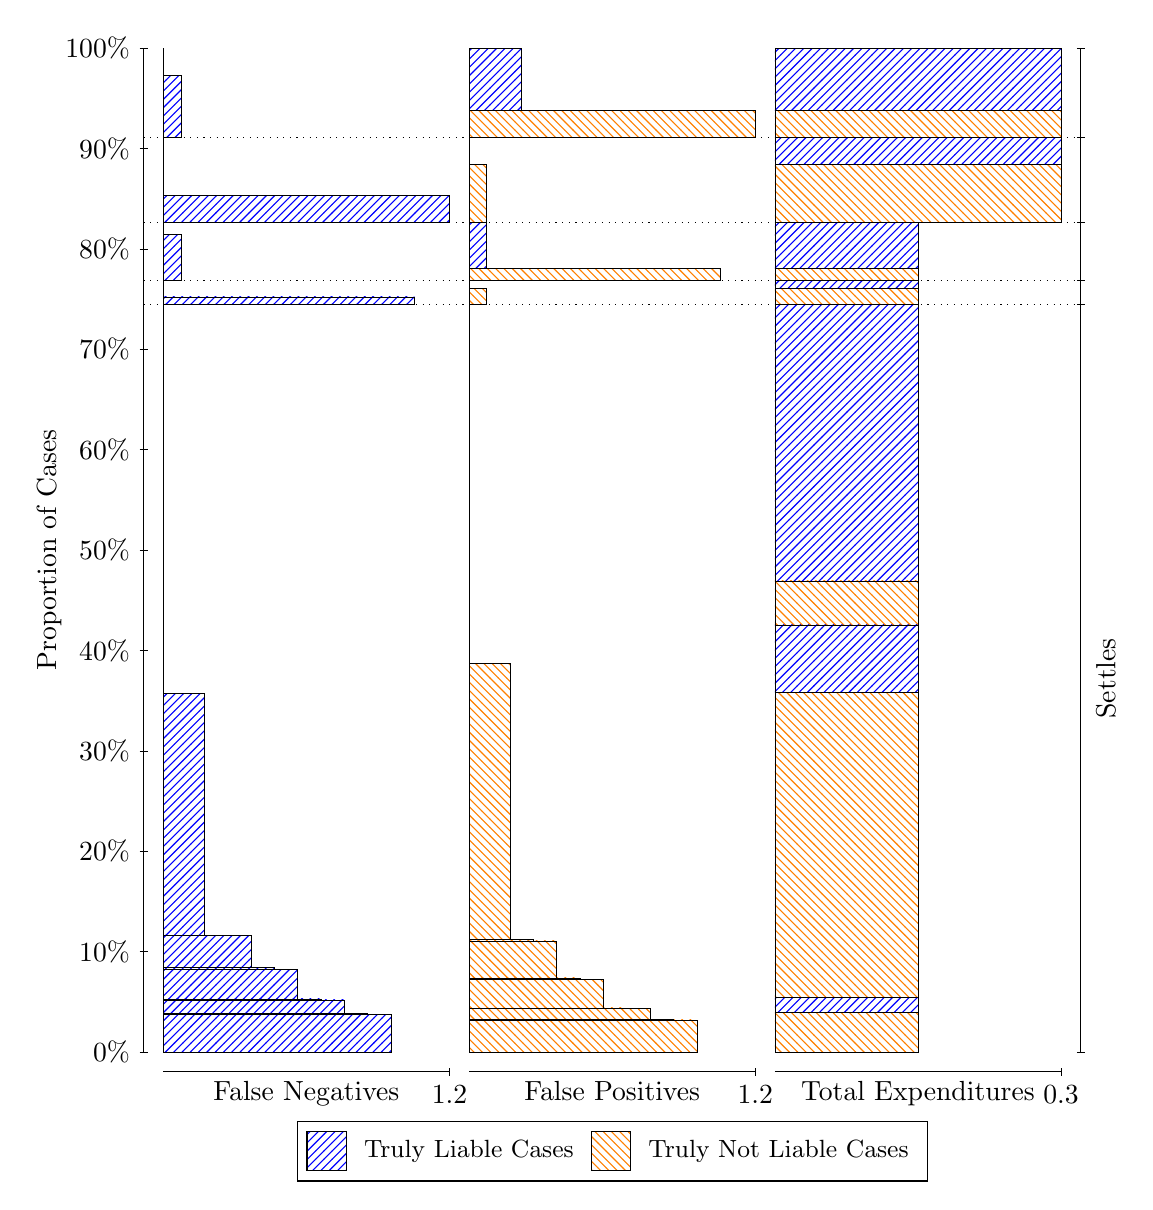
\begin{tikzpicture}
\draw[black, very thin] (1.5,1.75) -- (1.5,14.5);
\node[rotate=90, anchor=center] at (0.3, 8.125) {Proportion of Cases};
\draw[black, very thin] (1.45,1.75) -- (1.55,1.75);
\node[anchor=east] at (1.45, 1.75) {0\%};
\draw[black, very thin] (1.45,3.025) -- (1.55,3.025);
\node[anchor=east] at (1.45, 3.025) {10\%};
\draw[black, very thin] (1.45,4.3) -- (1.55,4.3);
\node[anchor=east] at (1.45, 4.3) {20\%};
\draw[black, very thin] (1.45,5.575) -- (1.55,5.575);
\node[anchor=east] at (1.45, 5.575) {30\%};
\draw[black, very thin] (1.45,6.85) -- (1.55,6.85);
\node[anchor=east] at (1.45, 6.85) {40\%};
\draw[black, very thin] (1.45,8.125) -- (1.55,8.125);
\node[anchor=east] at (1.45, 8.125) {50\%};
\draw[black, very thin] (1.45,9.4) -- (1.55,9.4);
\node[anchor=east] at (1.45, 9.4) {60\%};
\draw[black, very thin] (1.45,10.675) -- (1.55,10.675);
\node[anchor=east] at (1.45, 10.675) {70\%};
\draw[black, very thin] (1.45,11.95) -- (1.55,11.95);
\node[anchor=east] at (1.45, 11.95) {80\%};
\draw[black, very thin] (1.45,13.225) -- (1.55,13.225);
\node[anchor=east] at (1.45, 13.225) {90\%};
\draw[black, very thin] (1.45,14.5) -- (1.55,14.5);
\node[anchor=east] at (1.45, 14.5) {100\%};

\draw[black, very thin] (13.4,1.75) -- (13.4,14.5);
\draw[black, very thin] (13.35,1.75) -- (13.45,1.75);
\node[anchor=west] at (13.35, 1.75) {};
\draw[black, very thin] (13.35,11.241) -- (13.45,11.241);
\node[anchor=west] at (13.35, 11.241) {};
\draw[black, very thin] (13.35,11.546) -- (13.45,11.546);
\node[anchor=west] at (13.35, 11.546) {};
\draw[black, very thin] (13.35,12.285) -- (13.45,12.285);
\node[anchor=west] at (13.35, 12.285) {};
\draw[black, very thin] (13.35,13.368) -- (13.45,13.368);
\node[anchor=west] at (13.35, 13.368) {};
\draw[black, very thin] (13.35,14.5) -- (13.45,14.5);
\node[anchor=west] at (13.35, 14.5) {};

\draw[black, very thin, pattern color=blue, pattern=north east lines] (1.75,1.75) rectangle (4.6418,2.2297);
\draw[black, very thin, pattern color=blue, pattern=north east lines] (1.75,2.2297) rectangle (4.3452,2.2405);
\draw[black, very thin, pattern color=blue, pattern=north east lines] (1.75,2.2405) rectangle (4.0486,2.412);
\draw[black, very thin, pattern color=blue, pattern=north east lines] (1.75,2.412) rectangle (3.752,2.425);
\draw[black, very thin, pattern color=blue, pattern=north east lines] (1.75,2.425) rectangle (3.4554,2.8012);
\draw[black, very thin, pattern color=blue, pattern=north east lines] (1.75,2.8012) rectangle (3.1588,2.8236);
\draw[black, very thin, pattern color=blue, pattern=north east lines] (1.75,2.8236) rectangle (2.8622,3.227);
\draw[black, very thin, pattern color=blue, pattern=north east lines] (1.75,3.227) rectangle (2.5656,3.2324);
\draw[black, very thin, pattern color=blue, pattern=north east lines] (1.75,3.2324) rectangle (2.269,6.3084);
\draw[black, very thin, pattern color=orange, pattern=north west lines] (1.75,6.3084) rectangle (1.75,11.241);
\draw[black, very thin, pattern color=blue, pattern=north east lines] (1.75,11.241) rectangle (4.9384,11.339);
\draw[black, very thin, pattern color=orange, pattern=north west lines] (1.75,11.339) rectangle (1.75,11.546);
\draw[black, very thin, pattern color=blue, pattern=north east lines] (1.75,11.546) rectangle (1.9724,12.133);
\draw[black, very thin, pattern color=orange, pattern=north west lines] (1.75,12.133) rectangle (1.75,12.285);
\draw[black, very thin, pattern color=blue, pattern=north east lines] (1.75,12.285) rectangle (5.3833,12.627);
\draw[black, very thin, pattern color=orange, pattern=north west lines] (1.75,12.627) rectangle (1.75,13.368);
\draw[black, very thin, pattern color=blue, pattern=north east lines] (1.75,13.368) rectangle (1.9724,14.157);
\draw[black, very thin, pattern color=orange, pattern=north west lines] (1.75,14.157) rectangle (1.75,14.5);
\draw[black, very thin, pattern color=orange, pattern=north west lines] (5.6333,1.75) rectangle (8.5252,2.1572);
\draw[black, very thin, pattern color=orange, pattern=north west lines] (5.6333,2.1572) rectangle (8.2286,2.1591);
\draw[black, very thin, pattern color=orange, pattern=north west lines] (5.6333,2.1591) rectangle (7.932,2.2994);
\draw[black, very thin, pattern color=orange, pattern=north west lines] (5.6333,2.2994) rectangle (7.6354,2.3092);
\draw[black, very thin, pattern color=orange, pattern=north west lines] (5.6333,2.3092) rectangle (7.3388,2.6735);
\draw[black, very thin, pattern color=orange, pattern=north west lines] (5.6333,2.6735) rectangle (7.0422,2.6755);
\draw[black, very thin, pattern color=orange, pattern=north west lines] (5.6333,2.6755) rectangle (7.0422,2.691);
\draw[black, very thin, pattern color=orange, pattern=north west lines] (5.6333,2.691) rectangle (6.7456,3.1607);
\draw[black, very thin, pattern color=orange, pattern=north west lines] (5.6333,3.1607) rectangle (6.449,3.1761);
\draw[black, very thin, pattern color=orange, pattern=north west lines] (5.6333,3.1761) rectangle (6.1524,6.6824);
\draw[black, very thin, pattern color=blue, pattern=north east lines] (5.6333,6.6824) rectangle (5.6333,11.241);
\draw[black, very thin, pattern color=orange, pattern=north west lines] (5.6333,11.241) rectangle (5.8558,11.448);
\draw[black, very thin, pattern color=blue, pattern=north east lines] (5.6333,11.448) rectangle (5.6333,11.546);
\draw[black, very thin, pattern color=orange, pattern=north west lines] (5.6333,11.546) rectangle (8.8218,11.698);
\draw[black, very thin, pattern color=blue, pattern=north east lines] (5.6333,11.698) rectangle (5.8558,12.285);
\draw[black, very thin, pattern color=orange, pattern=north west lines] (5.6333,12.285) rectangle (5.8558,13.026);
\draw[black, very thin, pattern color=blue, pattern=north east lines] (5.6333,13.026) rectangle (5.6333,13.368);
\draw[black, very thin, pattern color=orange, pattern=north west lines] (5.6333,13.368) rectangle (9.2667,13.711);
\draw[black, very thin, pattern color=blue, pattern=north east lines] (5.6333,13.711) rectangle (6.3007,14.5);
\draw[black, very thin, pattern color=orange, pattern=north west lines] (9.5167,1.75) rectangle (11.333,2.2526);
\draw[black, very thin, pattern color=blue, pattern=north east lines] (9.5167,2.2526) rectangle (11.333,2.4479);
\draw[black, very thin, pattern color=orange, pattern=north west lines] (9.5167,2.4479) rectangle (11.333,6.3184);
\draw[black, very thin, pattern color=blue, pattern=north east lines] (9.5167,6.3184) rectangle (11.333,7.1743);
\draw[black, very thin, pattern color=orange, pattern=north west lines] (9.5167,7.1743) rectangle (11.333,7.7335);
\draw[black, very thin, pattern color=blue, pattern=north east lines] (9.5167,7.7335) rectangle (11.333,11.241);
\draw[black, very thin, pattern color=orange, pattern=north west lines] (9.5167,11.241) rectangle (11.333,11.448);
\draw[black, very thin, pattern color=blue, pattern=north east lines] (9.5167,11.448) rectangle (11.333,11.546);
\draw[black, very thin, pattern color=orange, pattern=north west lines] (9.5167,11.546) rectangle (11.333,11.698);
\draw[black, very thin, pattern color=blue, pattern=north east lines] (9.5167,11.698) rectangle (11.333,12.285);
\draw[black, very thin, pattern color=orange, pattern=north west lines] (9.5167,12.285) rectangle (13.15,13.026);
\draw[black, very thin, pattern color=blue, pattern=north east lines] (9.5167,13.026) rectangle (13.15,13.368);
\draw[black, very thin, pattern color=orange, pattern=north west lines] (9.5167,13.368) rectangle (13.15,13.711);
\draw[black, very thin, pattern color=blue, pattern=north east lines] (9.5167,13.711) rectangle (13.15,14.5);
\draw[black, dotted] (1.5,11.241) -- (13.4,11.241);
\draw[black, dotted] (1.5,11.546) -- (13.4,11.546);
\draw[black, dotted] (1.5,12.285) -- (13.4,12.285);
\draw[black, dotted] (1.5,13.368) -- (13.4,13.368);
\draw[black, very thin] (1.75,1.5) -- (5.3833,1.5);
\node[anchor=north] at (3.5667, 1.5) {False Negatives};
\draw[black, very thin] (5.3833,1.45) -- (5.3833,1.55);
\node[anchor=north] at (5.3833, 1.45) {1.2};

\draw[black, very thin] (5.6333,1.5) -- (9.2667,1.5);
\node[anchor=north] at (7.45, 1.5) {False Positives};
\draw[black, very thin] (9.2667,1.45) -- (9.2667,1.55);
\node[anchor=north] at (9.2667, 1.45) {1.2};

\draw[black, very thin] (9.5167,1.5) -- (13.15,1.5);
\node[anchor=north] at (11.333, 1.5) {Total Expenditures};
\draw[black, very thin] (13.15,1.45) -- (13.15,1.55);
\node[anchor=north] at (13.15, 1.45) {0.3};

\node[black, centered, rotate=90] at (13.72, 6.4954) {Settles};





\draw (7.449999999999999,1.5) node[draw=none] (baseCoordinate) {};
\begin{scope}[align=center]
        \matrix[scale=0.5, draw=black, below=0.5cm of baseCoordinate, nodes={draw}, column sep=0.1cm]{
            \node[rectangle, draw, minimum width=0.5cm, minimum height=0.5cm, pattern=north east lines, pattern color=blue] {}; &
            \node[draw=none, font=\small] (B) {Truly Liable Cases}; &
            \node[rectangle, draw, minimum width=0.5cm, minimum height=0.5cm, pattern=north west lines, pattern color=orange] {}; &
            \node[draw=none, font=\small] (B) {Truly Not Liable Cases}; \\
            };
\end{scope}

\end{tikzpicture}
\end{document}